\documentclass[hyperref=colorlinks]{beamer}
\mode<presentation>
\usetheme{iclpt}
\setbeamertemplate{navigation symbols}{}
\setbeamertemplate{headline}{
\begin{beamercolorbox}[leftskip=.2cm,rightskip=.2cm,topskip=.2cm,ht=1.1cm,dp=0.1cm,wd=\textwidth]{institute in head/foot}
  
\includegraphics[height=1cm]{icl.pdf}
  \hfill
  
\includegraphics[height=1cm]{../Pics/CMS-Color.pdf}
\end{beamercolorbox}
}
\setbeamertemplate{footline}{
\begin{beamercolorbox}[ht=.55cm,dp=0.4cm,wd=\textwidth,leftskip=.3cm]{author in head/foot}%
  \begin{minipage}[c]{5cm}%
    \usebeamerfont{author in head/foot}
    \insertshortauthor 
    \insertshorttitle
    \end{minipage}\hfill%
  \insertframenumber{} / \pageref{lastframe}
  \hfill
  \begin{minipage}{6cm}
    \hfill
  \end{minipage}
\end{beamercolorbox}%
}

\usepackage{color}
\usepackage{tabularx,colortbl}
\usepackage{graphicx}
\usepackage{pdfpages}
\usepackage{feynmp}
\DeclareGraphicsRule{*}{mps}{*}{}

\title{\vspace{-0.2cm} Combination of Higgs to Invisible Direct Measurements}
\subtitle{HIG-13-030 \vspace{-0.7cm}}
\author[P. Dunne]{\underline{P. Dunne} \\ on behalf of the H$\rightarrow$invisible analysis groups} % A.M. Magnan and A. Nikitenko Joao Pela with \\ R. Aggleton, J. Brooke: Bristol \\ C.Asawangtrakuldee, Q.Li: Peking \\ P. Srimanobhas: Chulalongkorn \\ S. Kumar, K. Mazumdar: Mumbai}
\titlegraphic{
  \vspace{-0.7cm}
  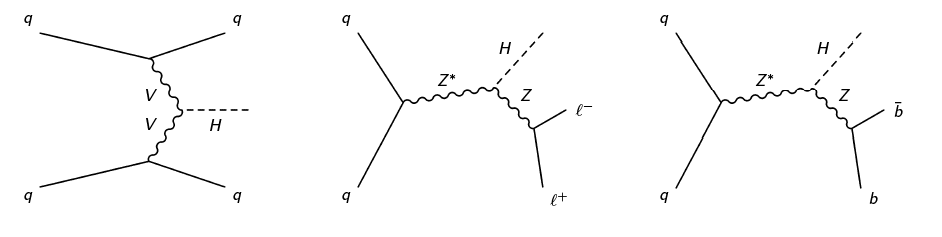
\includegraphics[width=\textwidth]{TalkPics/invcomb021213/feyndiags}
%% \begin{fmfgraph*}(100,70)
%%         \fmfleft{i1,i2}
%%         \fmfright{o1,o2,o3}
%%         \fmf{fermion}{i1,v1,o1}
%%         \fmf{fermion}{i2,v2,o3}
%%         \fmf{phantom,tension=4/5}{v1,v2}
%%         \fmffreeze
%%         \fmf{photon,label=$W,,Z$}{v1,v3}
%%         \fmf{photon,label=$W,,Z$}{v2,v3}
%%         \fmf{dashes}{v3,o2}
%%         \fmflabel{$q$}{i1}
%%         \fmflabel{$q$}{i2}
%%         \fmflabel{$q$}{o1}
%%         \fmflabel{$q$}{o3}
%%         \fmflabel{$H$}{o2}
%%       \end{fmfgraph*}
}
\date{}
\begin{document}
\begin{fmffile}{feynmandiags}

%TITLE PAGE
\section{Title}
\begin{frame}
  \titlepage
  
\end{frame}

%OUTLINE
\begin{frame}
  \frametitle{Introduction}
  \begin{itemize}
  \item Many BSM theories predict invisible final states of the Higgs:
  \item[-] SUSY, Extra Dimensions, etc.
  \item Direct searches must be performed in the associated production channels
  \item There are currently three approved CMS Higgs to invisible results in the following channels:
  \item[-] VBF (HIG-13-013), Z($\ell\ell$)H(inv) (HIG-13-018), Z($b\bar{b}$)H(inv) (HIG-13-028)
  \item These results have been combined for a paper (HIG-13-030)
  \end{itemize}
\end{frame}

\begin{frame}
  \frametitle{Indirect Result from Visible Decays}
  \centering
  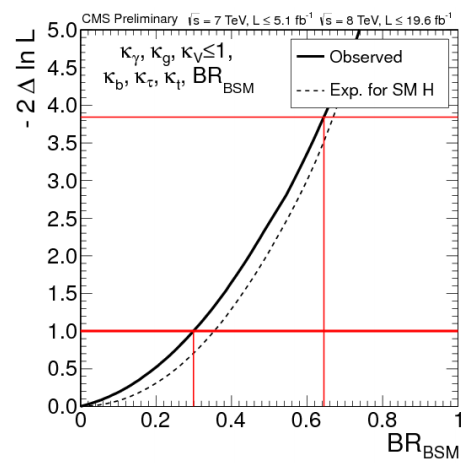
\includegraphics[height=.6\textheight]{indirectbrbsm.png}
  \begin{itemize}
  \item Observed (expected) limit of 64\% (67\%) at 95\% C.L. on $BR_{inv} $ for a 125 GeV Higgs (HIG-13-005)
  \item[-] Combination between direct and indirect methods is being investigated e.g. \href{https://indico.cern.ch/getFile.py/access?contribId=3&sessionId=9&resId=1&materialId=slides&confId=267834}{talk by M. Zanetti}
  \end{itemize}
\end{frame}

\begin{frame}
  \frametitle{Datacards}
  \begin{itemize}
    \item All three channels have signal MC at different mass points
  \end{itemize}
  \begin{center}
  \begin{tabular}{|l|c|}
    \hline
    Channel & Mass Points/GeV \\
    \hline
    Z($\ell\ell$)H(inv) & 105, 115, 125, 135, 145, 175, 200 \& 300 \\
    Z($b\bar{b}$)H(inv) & 105, 115, 125, 135, 145 \& 150 \\
    VBF & 110, 125, 150, 200, 300 \& 400 \\
    \hline
  \end{tabular}
  \end{center}
  \begin{itemize}
  \item New VBF datacards were produced for 115,135 and 145 GeV
  \item[-] Nuisances are linearly interpolated between mass points.
  \item[-] Signal yields are interpolated using the method described below.
  \end{itemize}
\end{frame}  

\begin{frame}
  \frametitle{Signal Yield interpolation}
  \begin{columns}
    \column{.5\textwidth}
    \begin{itemize}
    \item $N_{Signal}=eff. \times acc. \times \mathcal L\sigma$
    \item Luminosity is constant
    \item Yield over cross-section is thus proportional to efficiency times acceptance
    \item[-] Cross-sections from LHC-HXSWG were used
    \end{itemize}
    \column{.5\textwidth}
    \centering
    \hspace{-.5cm}
    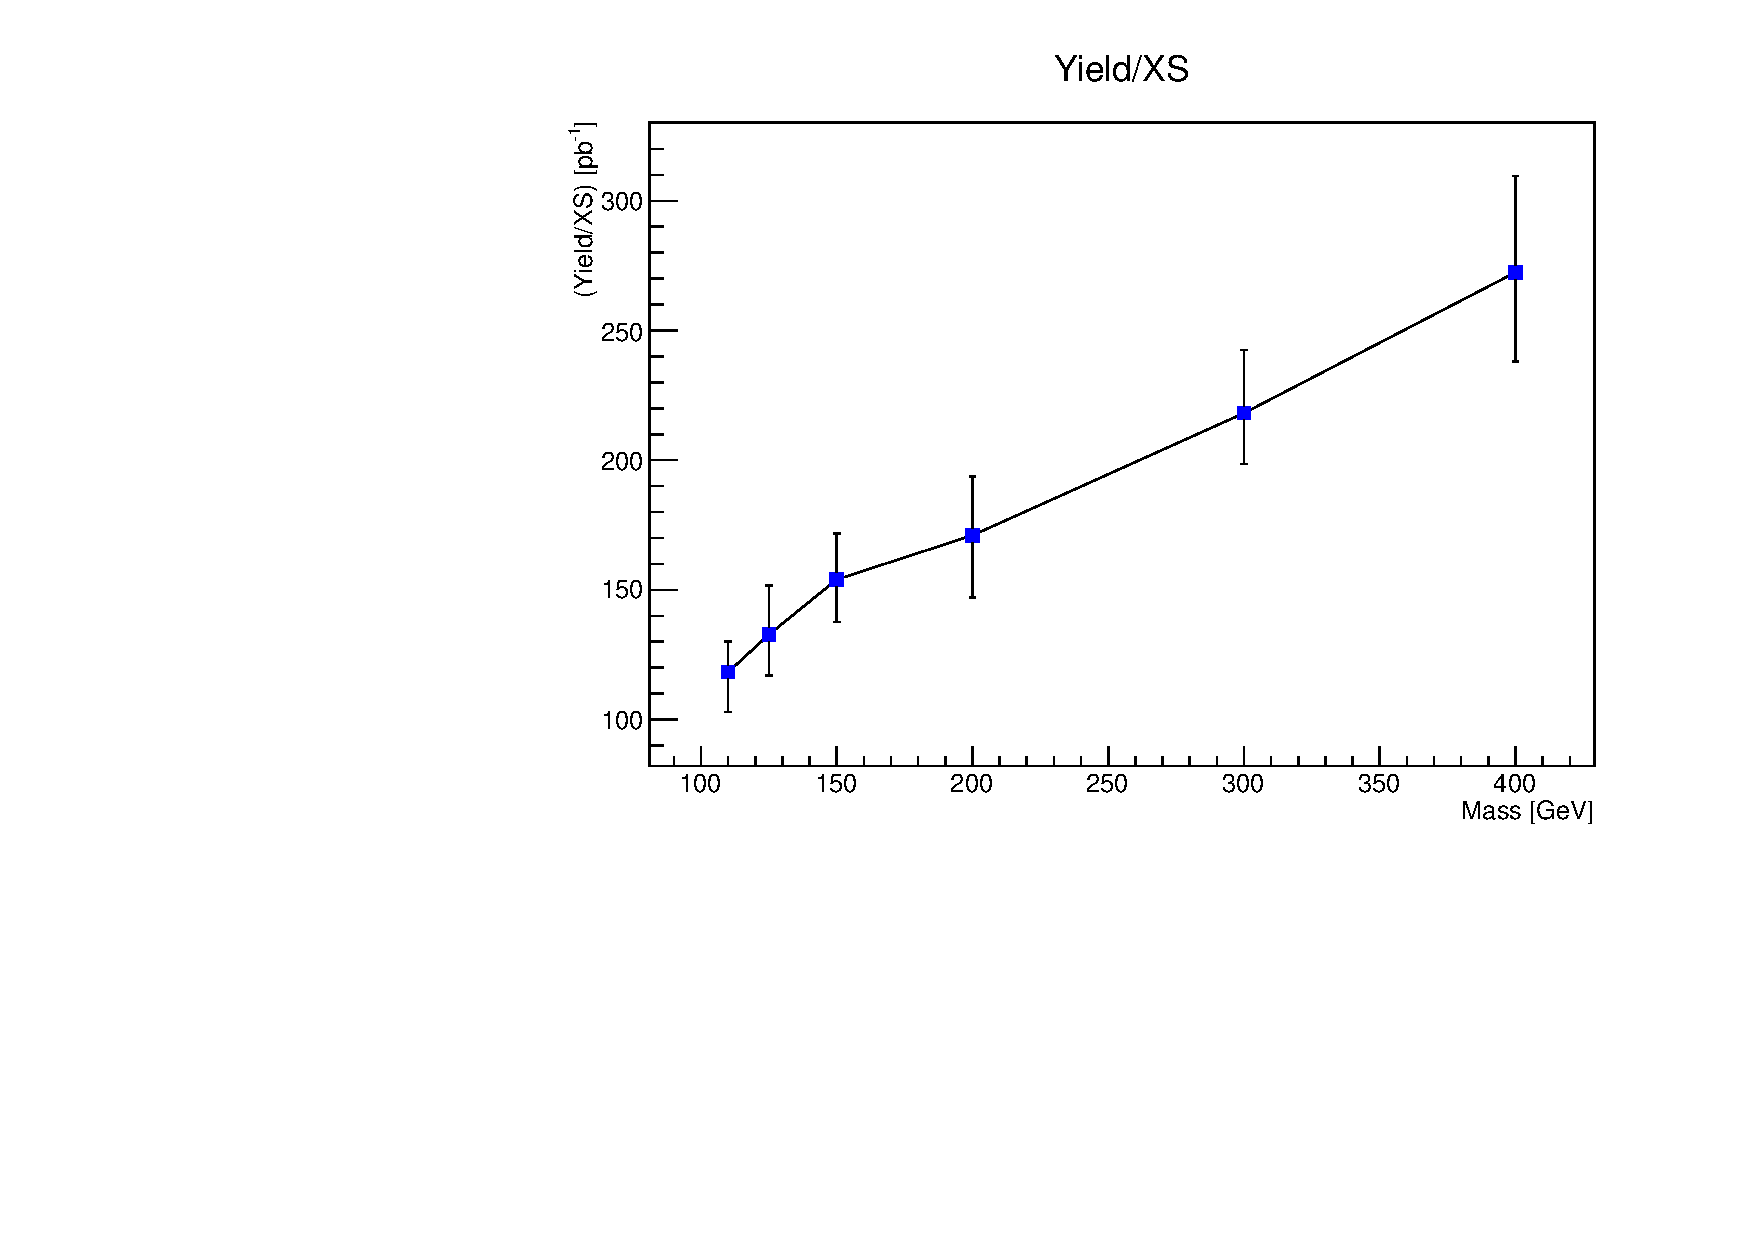
\includegraphics[clip=true,trim=0 0 0 30, width=1.2\textwidth]{TalkPics/invcomb021213/yieldoverxs.pdf}
  \end{columns}
\end{frame}

\begin{frame}
  \frametitle{Combination Method}
  \begin{itemize}
  \item The cards for the three channels were combined using the standard Higgs combination tool
  \item The following uncertainties were considered correlated between channels in decreasing order of importance:
  \end{itemize}
    \begin{tabular}{|l|c|}
      \hline
      Nuisance & Analyses which it affects \\
      \hline
      Jet energy scale & VBF, Z($\ell\ell$)H(inv) \\
      PDF uncertainties & VBF, Z($b\bar{b}$), Z($\ell\ell$)H(inv) \\
      QCD scale & VBF, Z($b\bar{b}$), Z($\ell\ell$)H(inv) \\
      Luminosity & VBF, Z($b\bar{b}$)H(inv), Z($\ell\ell$)H(inv) \\
      Jet energy resolution & VBF, Z($\ell\ell$)H(inv) \\
      Unclustered energy scale & VBF, Z($b\bar{b}$)H(inv), Z($\ell\ell$)H(inv) \\
      Muon identification efficiency & VBF, Z($\ell\ell$)H(inv) \\
      Electron identification efficiency & VBF, Z($\ell\ell$)H(inv) \\
      \hline
    \end{tabular}
\end{frame}
    
\begin{frame}
  \frametitle{Separate results: Direct}
  \centering
  \begin{columns}
    \column{.5\textwidth}
    \begin{itemize}
    \item VBF
    \end{itemize}
    \column{.5\textwidth}
    \begin{itemize}
    \item ZH
    \end{itemize}
  \end{columns}
  \begin{columns}
    \column{.5\textwidth}
    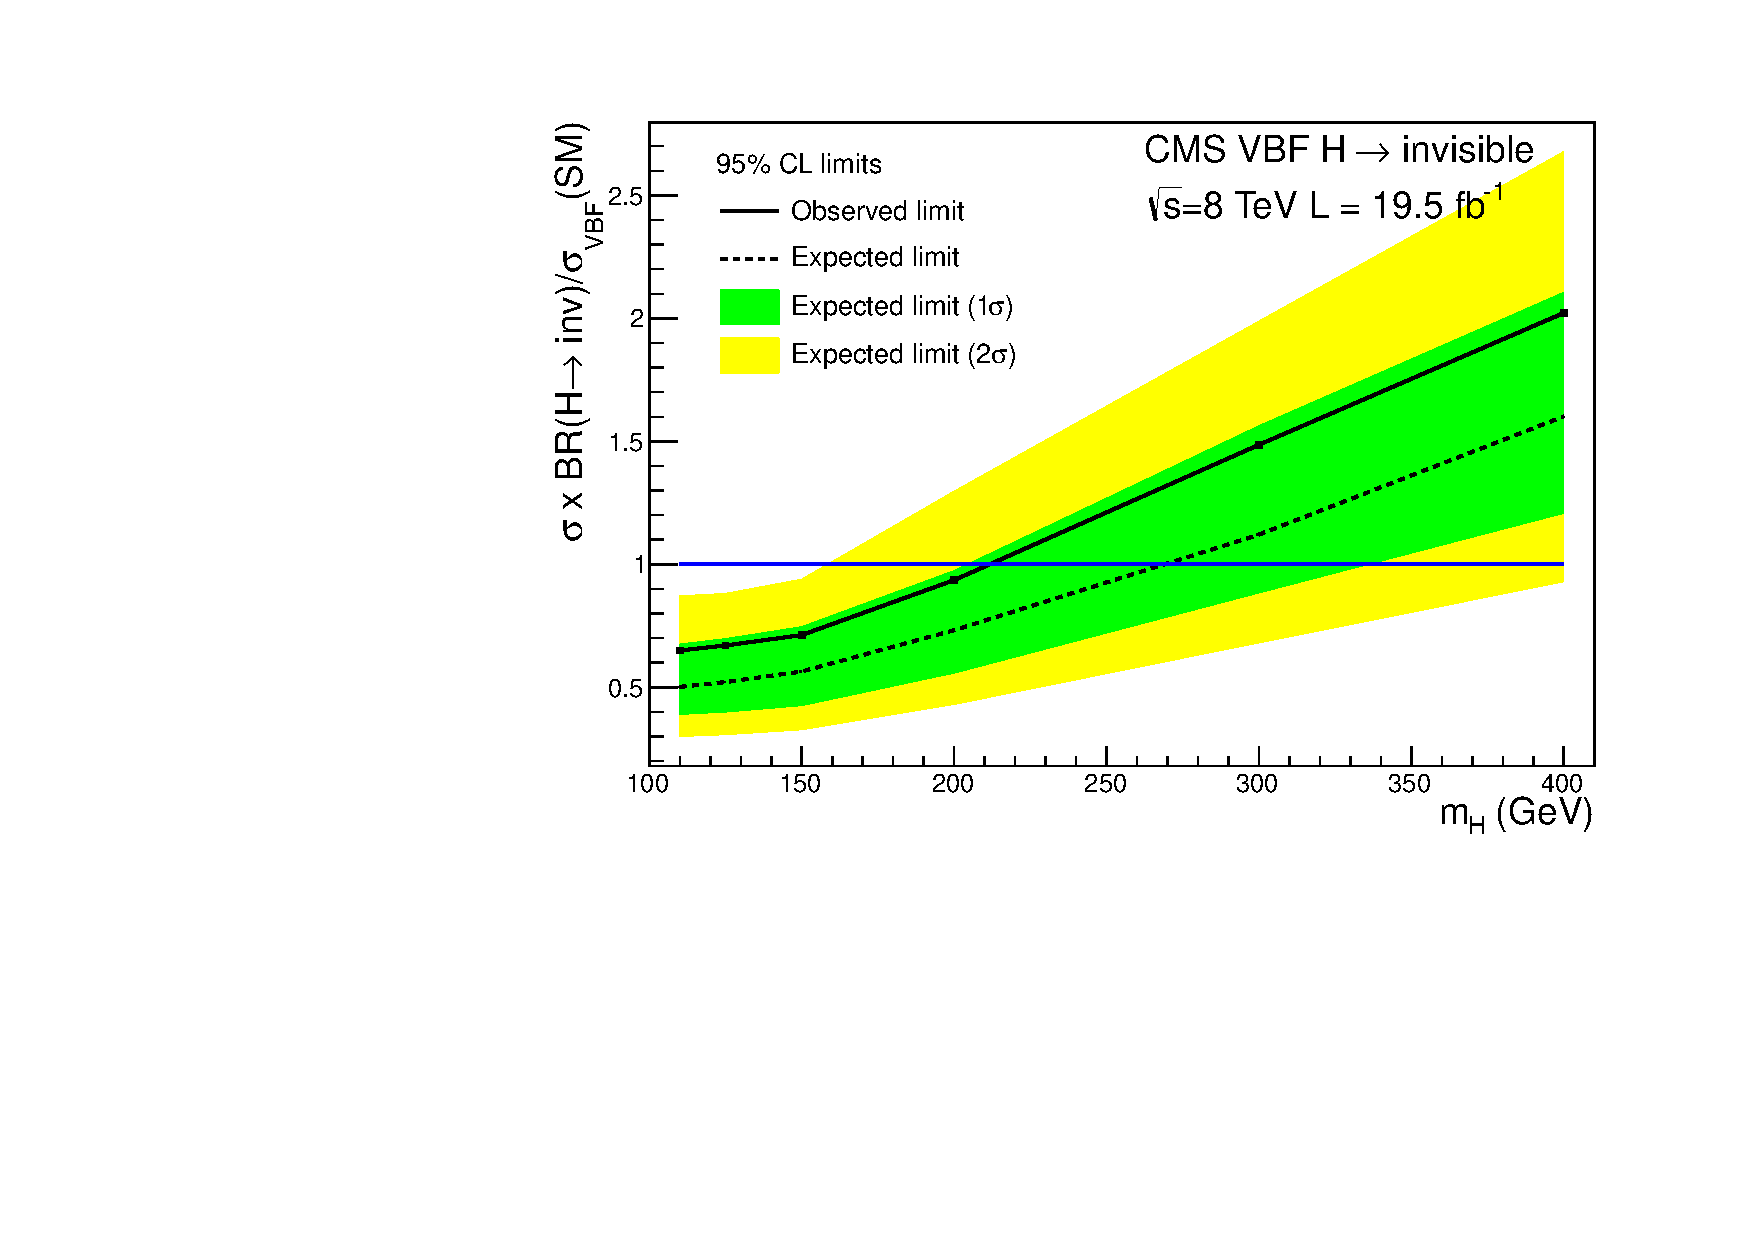
\includegraphics[width=\textwidth]{TalkPics/invcomb021213/vbflimit.pdf}
    \column{.5\textwidth}
    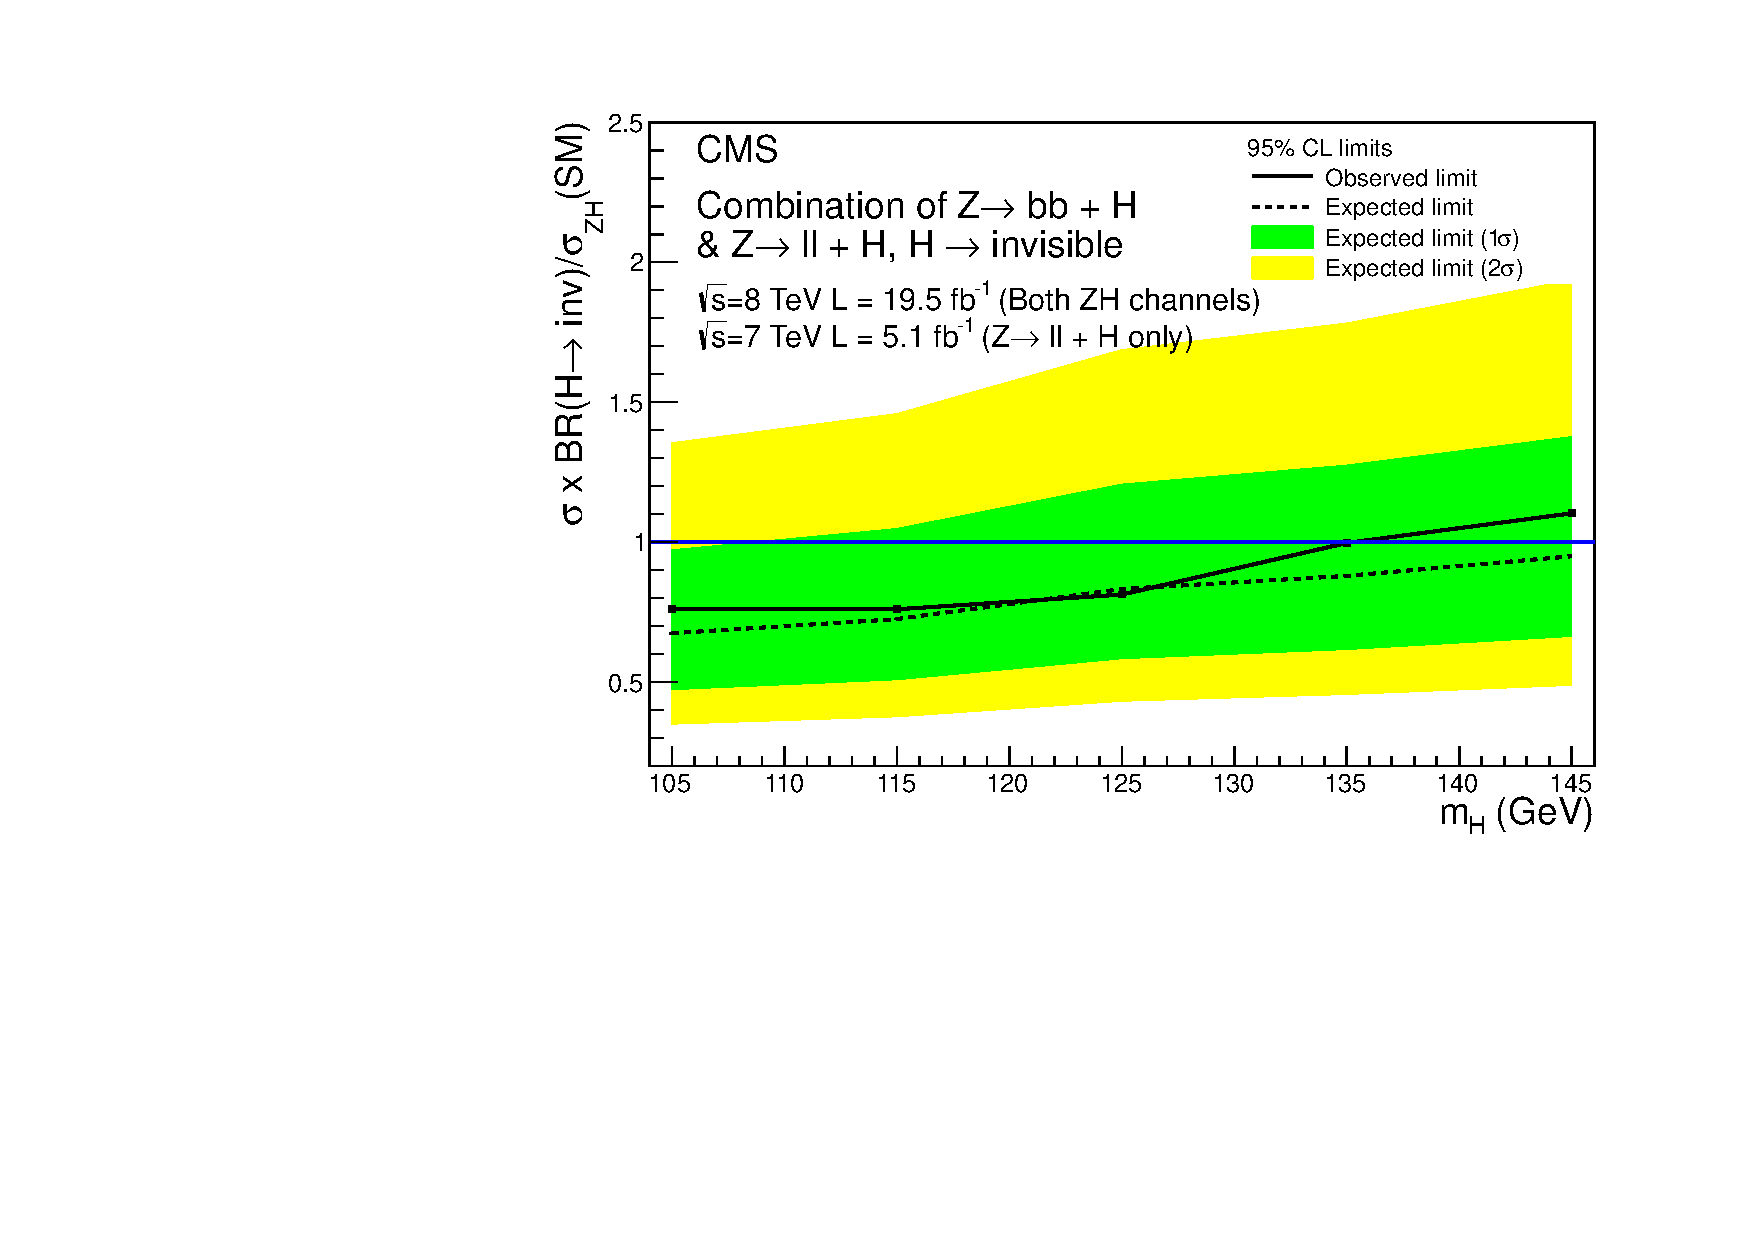
\includegraphics[width=\textwidth]{TalkPics/invcomb021213/zhlimit.pdf}
  \end{columns}
  \begin{columns}
    \column{.5\textwidth}
    \begin{itemize}
    \item Observed (expected) limit of 67\% (52\%) at 95\% C.L. on $BR_{inv}$ for a 125 GeV Higgs
    \end{itemize}
    \column{.5\textwidth}
    \begin{itemize}
    \item Observed (expected) limit of 81\% (83\%) at 95\% C.L. on $BR_{inv}$ for a 125 GeV Higgs
    \end{itemize}
  \end{columns}
\end{frame}

\begin{frame}
  \frametitle{Separate results: Cross-Section limits}
  \centering
  \begin{columns}
    \column{.5\textwidth}
    \begin{itemize}
    \item VBF
    \end{itemize}
    \column{.5\textwidth}
    \begin{itemize}
    \item ZH
    \end{itemize}
  \end{columns}
  \begin{columns}
    \column{.5\textwidth}
    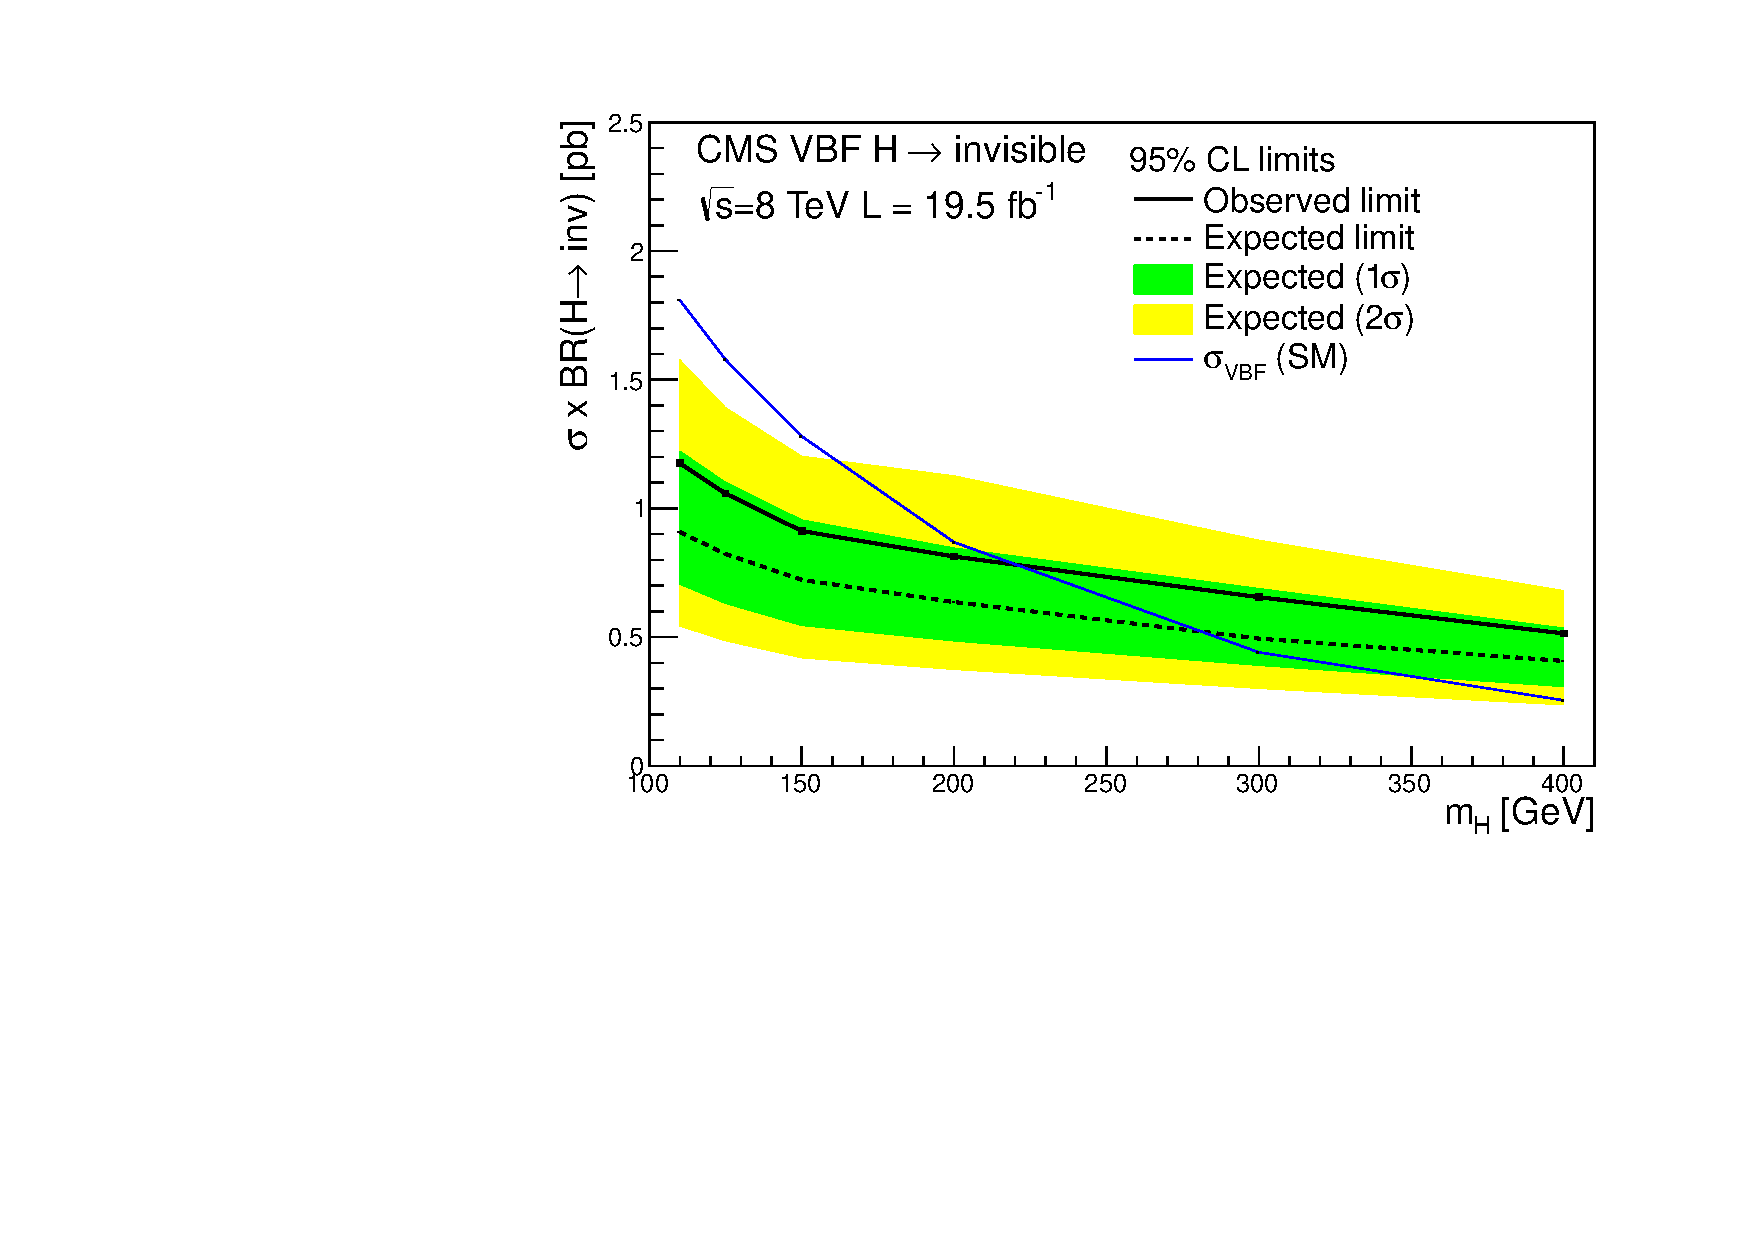
\includegraphics[width=\textwidth]{TalkPics/invcomb021213/vbfxslimit.pdf}
    \column{.5\textwidth}
    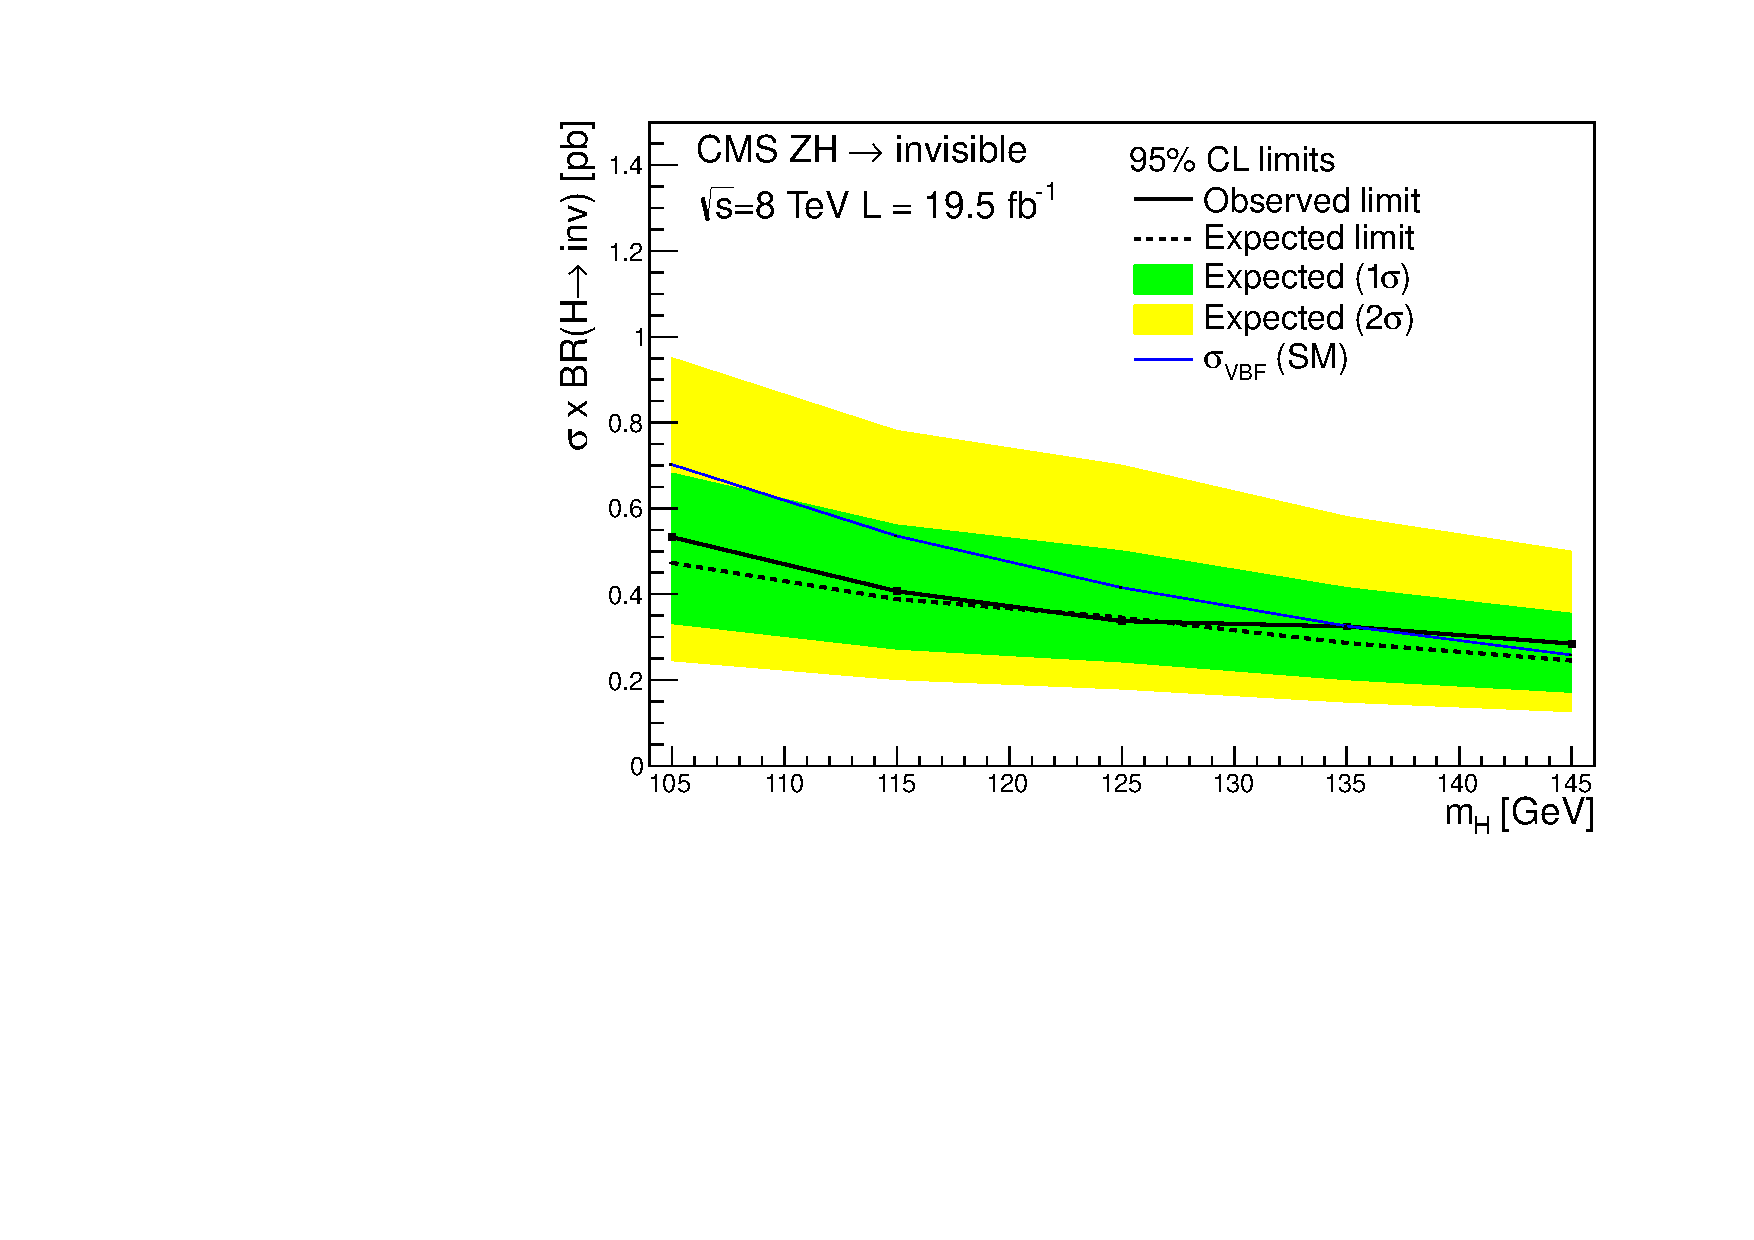
\includegraphics[width=\textwidth]{TalkPics/invcomb021213/zhxslimit.pdf}
  \end{columns}
  \begin{columns}
    \column{.5\textwidth}
    \begin{itemize}
    \item Observed (expected) limit of 67\% (52\%) at 95\% C.L. on $BR_{inv}$ for a 125 GeV Higgs
    \end{itemize}
    \column{.5\textwidth}
    \begin{itemize}
    \item Observed (expected) limit of 81\% (83\%) at 95\% C.L. on $BR_{inv}$ for a 125 GeV Higgs
    \end{itemize}
  \end{columns}
\end{frame}

\begin{frame}
  \frametitle{Combined Results}
  \centering
  \vspace{-.2cm}
  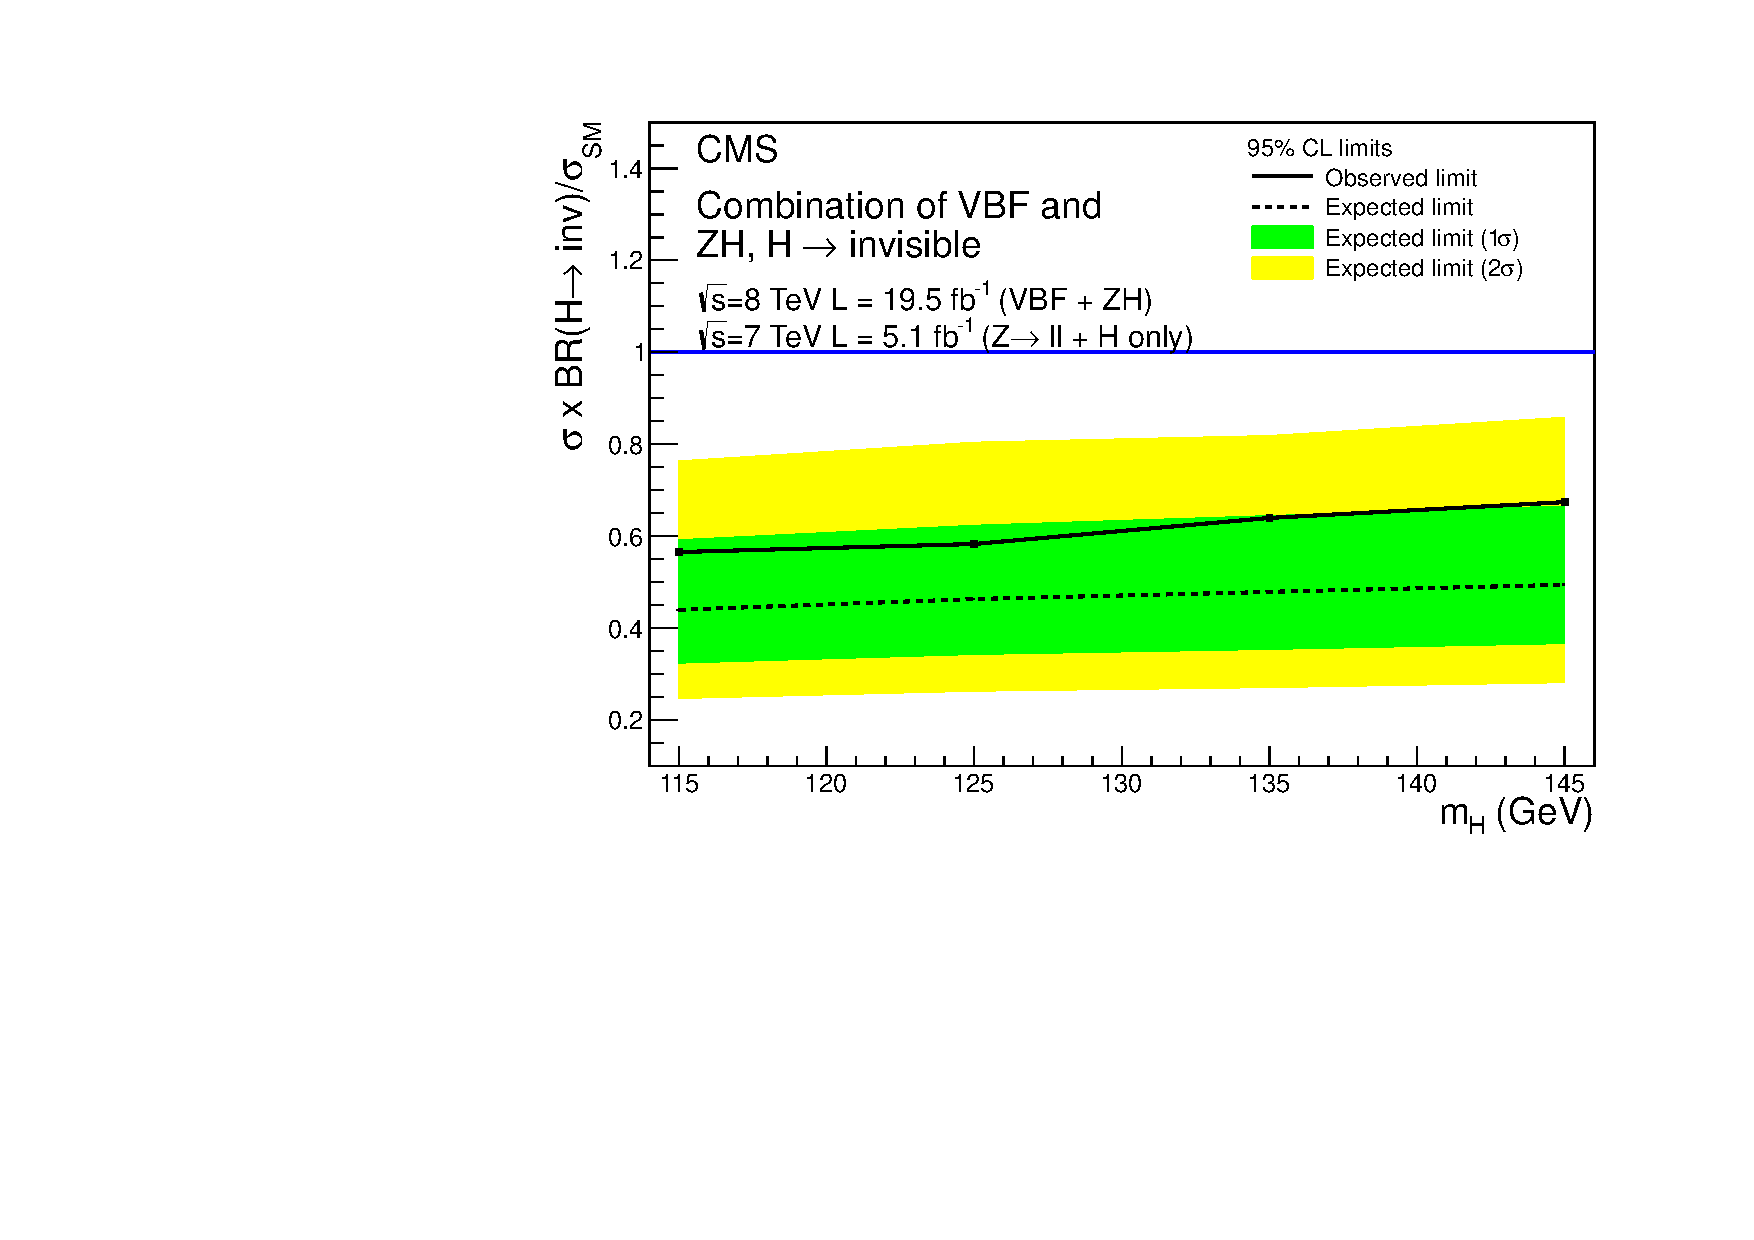
\includegraphics[clip=true,trim=0 5 0 20, width=.8\textwidth]{TalkPics/invcomb021213/combinedlimit.pdf}
  \vspace{-.3cm}
  \begin{itemize}
  \item Observed (expected) limit at 125 GeV is 58(46)\%
  \end{itemize}
\end{frame}

\begin{frame}
  \frametitle{High mass combination}
  \centering
  \vspace{-.3cm}
  \begin{itemize}
  \item Z($\ell\ell$)H(inv) and VBF both have datacards up to 300 GeV
  \item The same combination method as used above was used to combine these two channels between 115 and 300 GeV
  \end{itemize}
  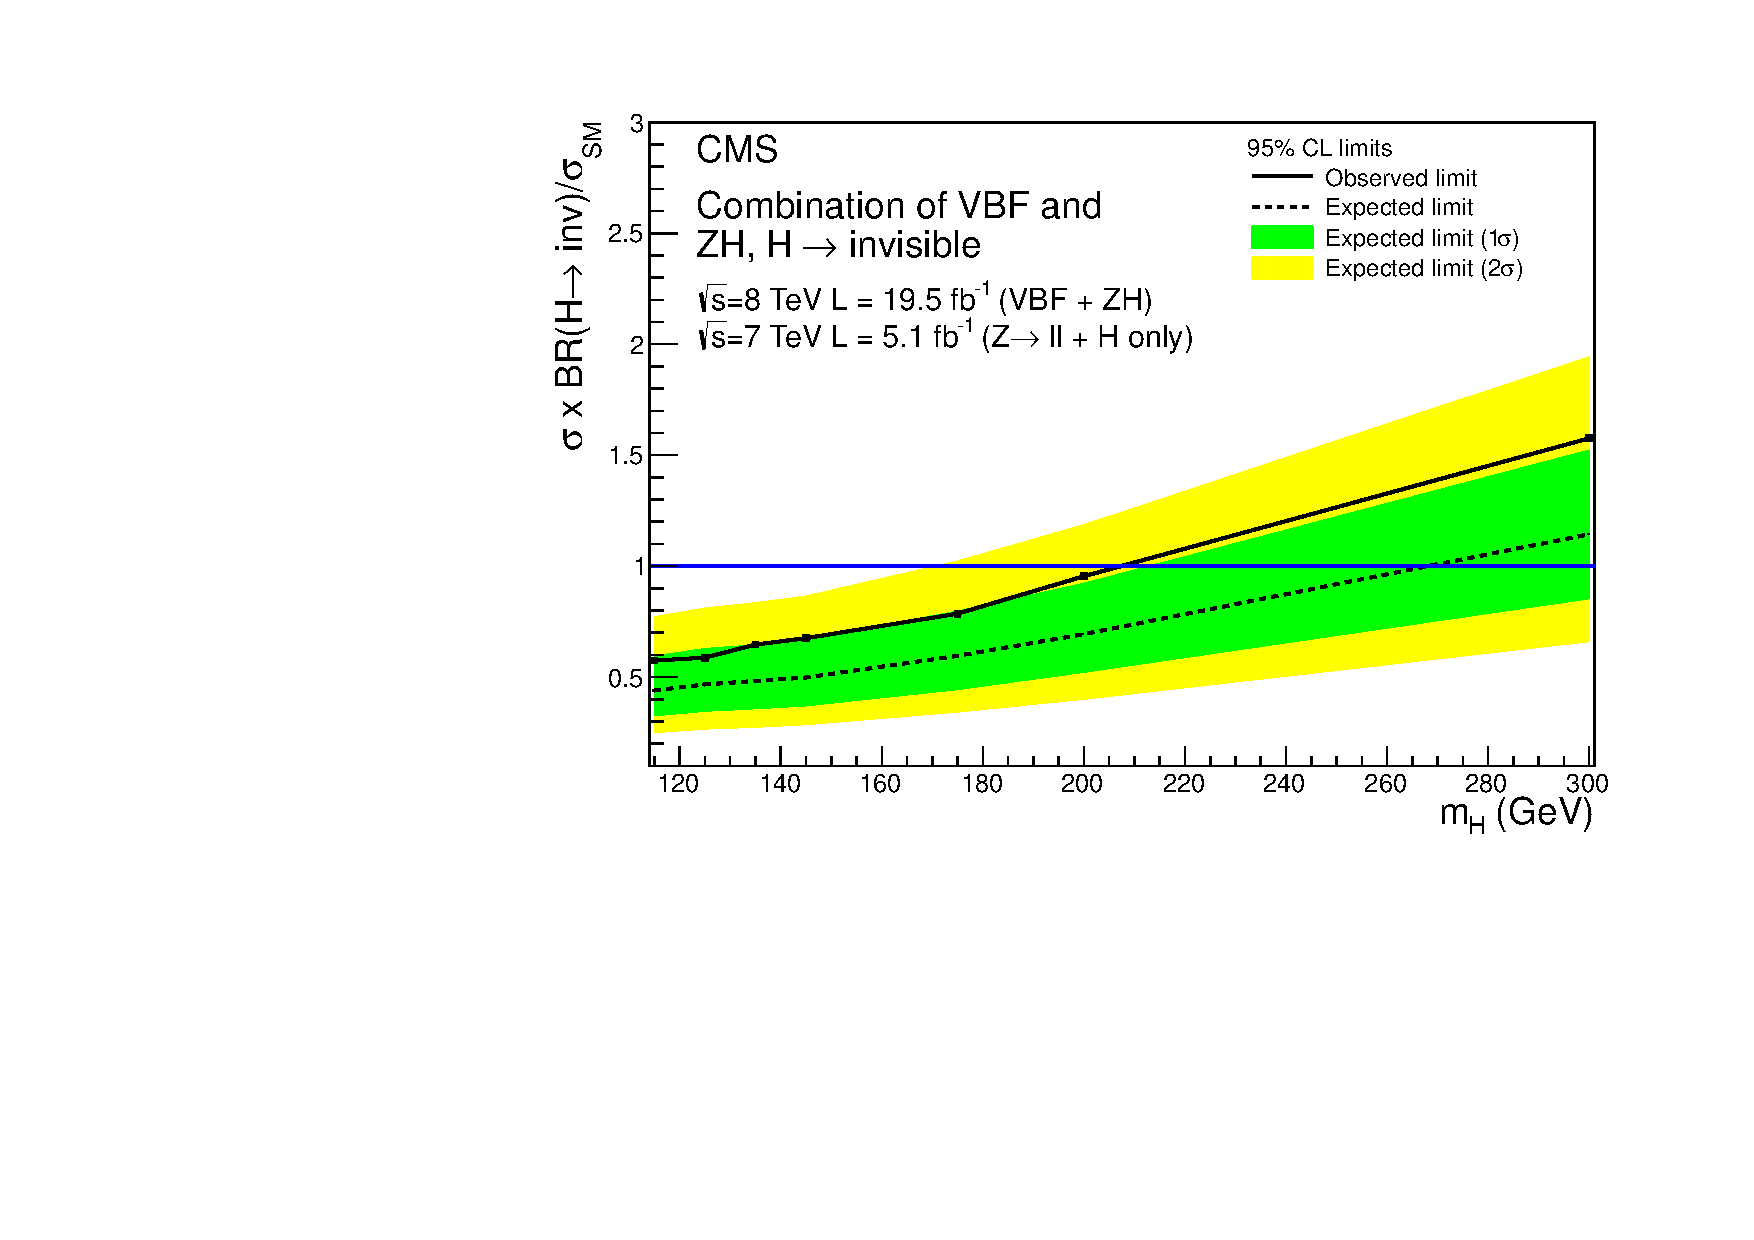
\includegraphics[clip=true,trim=0 5 0 20, width=.75\textwidth]{TalkPics/invcomb021213/highmasslimit.pdf}
 \end{frame}


\begin{frame}
  \frametitle{Conclusions}
  \label{lastframe}
  \begin{columns}
    \column{.5\textwidth}
    \begin{itemize}
    \item All three H$\rightarrow$invisible channels have been combined using the standard Higgs combination tool
    \item The result is compatible with the SM
    \item The combined result gives the strongest limit on the invisible branching fraction of the 125 GeV Higgs
    \end{itemize}
    \column{.5\textwidth}
    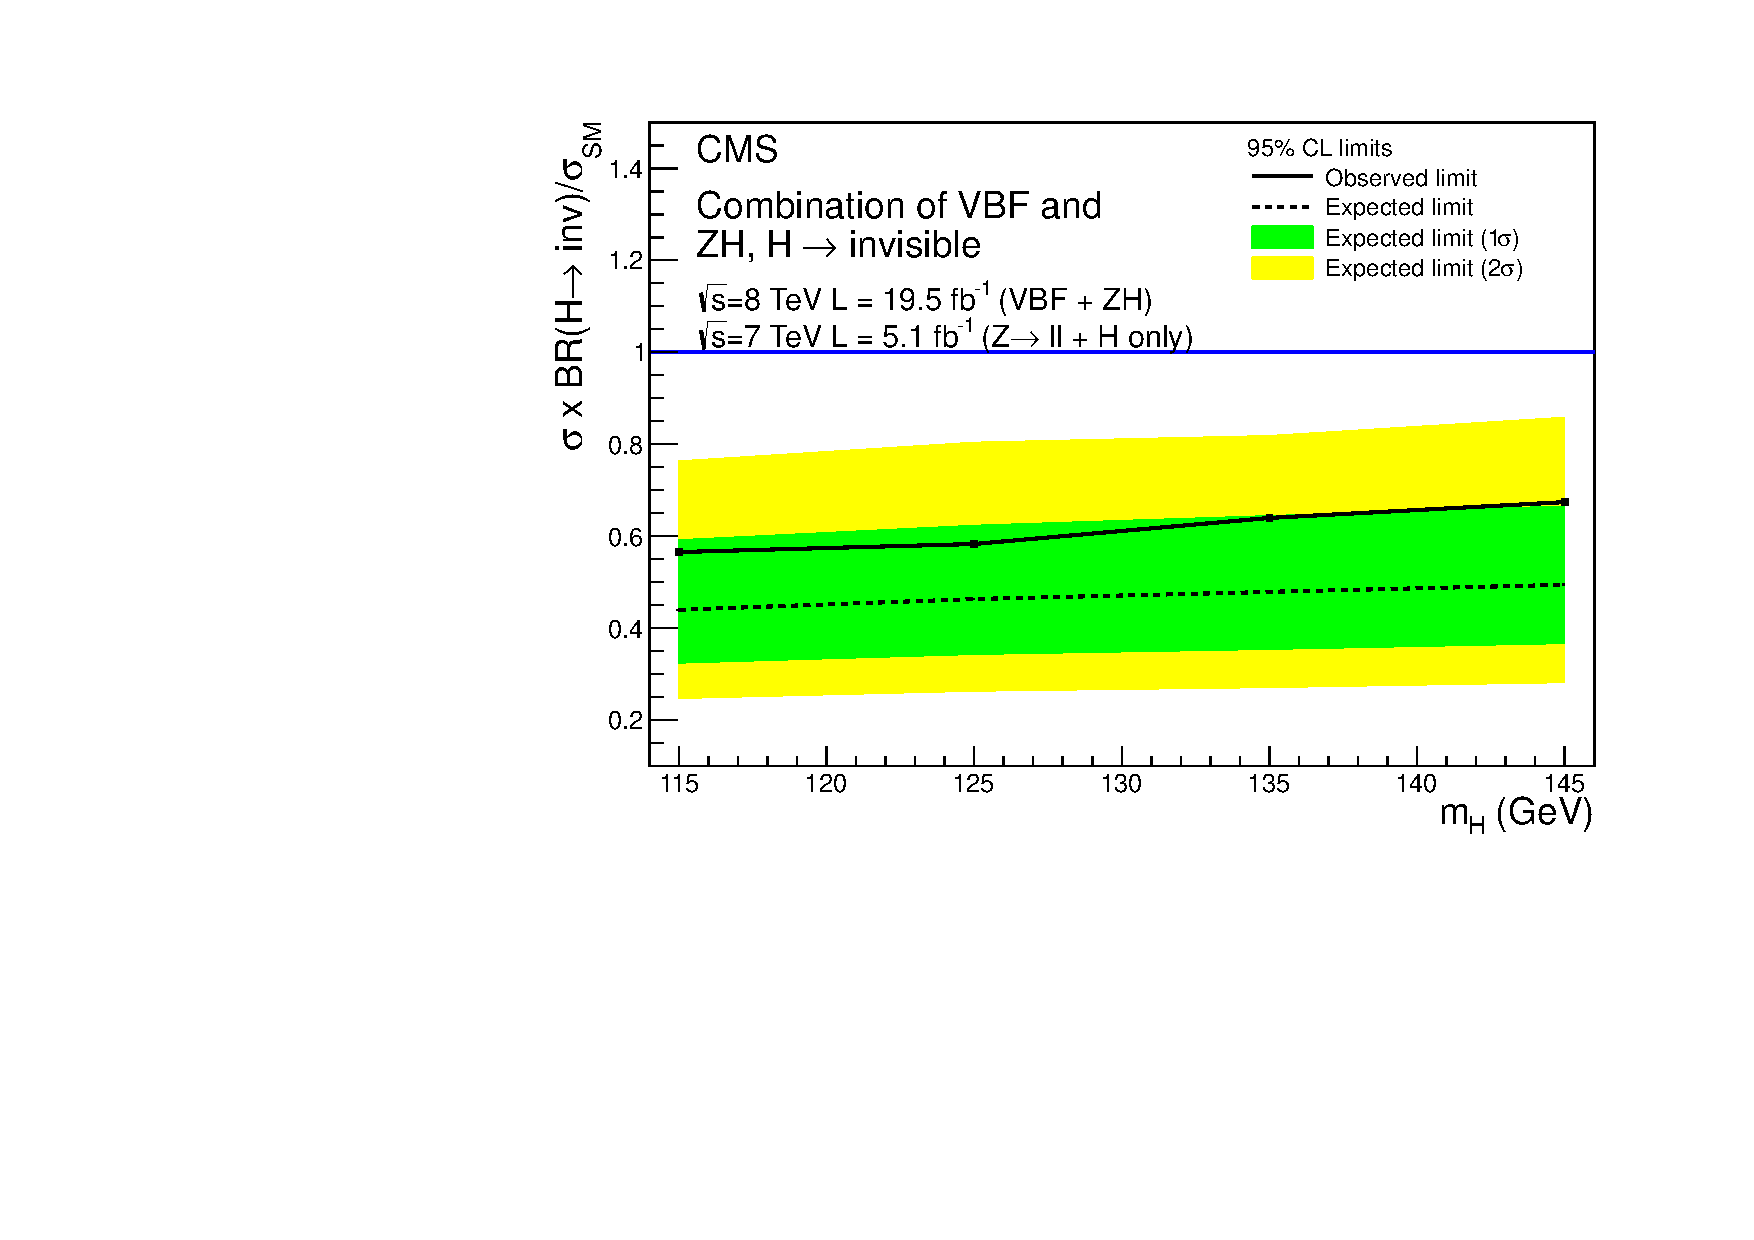
\includegraphics[clip=true,trim=0 5 0 20, width=1.2\textwidth]{TalkPics/invcomb021213/combinedlimit.pdf}
  
  \end{columns}
\end{frame}

\begin{frame}
  \frametitle{Backup}
\end{frame}

\begin{frame}
  \frametitle{Previous Limits}
  \begin{itemize}
  \item CMS PAS limits on $BR_{inv}$ for a 125 GeV Higgs boson are:
  \item[-] VBF: observed (expected) limit of 69\% (53\%) at 95\% C.L.
  \item[-] Z($\ell\ell$)H(inv): observed (expected) limit of 75\% (91\%) at 95\% C.L.
  \item[-] Z($b\bar{b}$)H(inv): ovserved (expected) limit of 182\% (199\%) at 95\% C.L.
  \item[-] CMS indirect limit, from visible channels: observed (expected) limit of 64\% (67\%) at 95\% C.L.
  \item ATLAS also produce an indirect limit and a limit in the ZH channel:
  \item[-] Indirect limit 60\% (no expected limit given)
  \item[-] ZH: observed (expected) 65\% (84\%)    
  \end{itemize}
\end{frame}

\begin{frame}
  \frametitle{VBF Cross-sections}
  \centering
  \begin{tabular}{|l|c|}
  \hline  
  Mass/GeV & $\sigma/pb$ \\
  \hline  
  110 & $1.809 \pm 0.048$\\
  115 & $1.729 \pm 0.046$\\
  125 & $1.578 \pm 0.042$\\
  135 & $1.448 \pm 0.038$\\
  145 & $1.333 \pm 0.035$\\
  150 & $1.280 \pm 0.033$\\
  200 & $0.869 \pm 0.023$\\
  300 & $0.441 \pm 0.011$\\
  400 & $0.254 \pm 0.007$\\
  \hline  
  \end{tabular}
\end{frame}

{
\setbeamercolor{background canvas}{bg=}
\includepdf[pages=31]{TalkPics/VBF-H-Invisible-Approval.pdf}
}

\end{fmffile}
\end{document}

